\documentclass[11pt,a4paper,oneside]{scrartcl}
\setlength{\parindent}{0pt}

\usepackage{fixltx2e}%% the official fixes for LaTeX2e
\usepackage[a4paper,left=1in, right=1in, top=1in, bottom=1in]{geometry}
\usepackage[draft]{graphicx} %% add [draft] for not generating figures (compiles much faster, in case only want to see text)
\usepackage{color}
\usepackage{float}
\usepackage{amsmath}
\usepackage{amssymb}
\usepackage{soul} %% use \hl to higlight text
\usepackage[section]{placeins} %% use \FloatBarrier command  to prevent floats to appear beyond some point in your documen


\newcommand\Rey{\mbox{\textit{Re}}\,\,}
\newcommand\bfr[1]{\textcolor[rgb]{1,0.00,0.00}{\textbf{\textsf{#1}}}}
\newcommand\ra{$\rightarrow$}
\newcommand\cm{\textcolor[rgb]{0.00,0.50,0.00}{\checkmark}\,\,}
\begin{document}

EG501V Computational Fluid Dynamics (2014/2015)
\\
\\
\textbf{Practical: CFD modeling of laminar and turbulent pipe flow using ANSYS Fluent}

\section{Introduction}
This tutorial shows how to solve the basic problem of fluid flow through a circular pipe. Two flow scenarios are considered: (1) laminar flow and (2) turbulent flow  through the pipe. In the laminar scenario we will solve the momentum equation directly and in the turbulent flow scenario we will use the $k-\varepsilon$ closure model, which was covered in lecture notes 8 on turbulence modeling.  The learning outcomes of this tutorial cover the four key elements involving  CFD analysis, which are setting up the \emph{Geometry} of your model, \emph{Mesh generation}, performing the \emph{Fluent analysis}  and \emph{Post-processing} of your results. The tutorial will guide you step-by-step through these four procedures and provide you with a basic skill set to complete your CFD design assignment.

\section{Laminar pipe flow}

\subsection{Problem description}
Consider a fluid flowing through a circular pipe of diameter $D$ and length $L$ as sketched below. The pipe diameter is $D=0.3$\,m and the length of the pipe is $L=6$\,m. The inlet velocity  is constant over the cross-section and is equal to $U=1$\,m/s. The  fluid density is $\rho=1$\,kg/m$^3$ and the fluid viscosity is $\mu=1.5\times10^{-3}$\,kg/ms. Note that these properties result in a Reynolds number of $\Rey=\rho DL/\mu=200$ which means the flow is laminar. The outlet pressure $p_\mathrm{o}$ is equal to 1 atmosphere (standard pressure).\\
\begin{center}
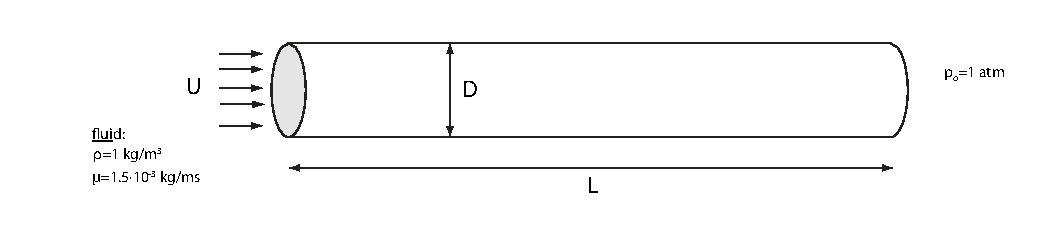
\includegraphics[width=\textwidth,clip]{pipe_sketch.pdf}
\end{center}
Solve this flow problem using ANSYS Fluent and present the following results:
\begin{itemize}
\item velocity vectors
\item velocity magnitude contours
%\item pressure contours
\item velocity profiles
\item skin friction coefficient along the pipe wall
\end{itemize}

Compare these results with the analytical solution for fully developed laminar pipe flow.


\subsection{Starting ANSYS workbench}

Prior to opening ANSYS, create a folder (e.g. FluentCFD) on your \emph{H:drive}. This folder will be used to store the files created during this session, and allow you to reopen them at a later stage. You will need approximately 10\,MB of free space for this tutorial, so make sure this space is available on your \emph{H:drive}.\\

On the desktop go to the folder \bfr{Physical Sciences\ra Engineering\ra ANSYS 14.5} and double click the shortcut \bfr{Workbench 14.5}, see the figure below.

\begin{figure}[H]
\begin{center}
\includegraphics[width=.8\textwidth,clip]{desktop.png}
\end{center}
\end{figure}

You should now see a window as in the figure below.

\begin{figure}[H]
\begin{center}
\includegraphics[width=.8\textwidth,clip]{workbench.png}
\end{center}
\end{figure}

This is the ANSYS workbench which consists primarily of the \emph{Toolbox area} (left column) and the \emph{Project schematic} in the main area. Above these areas you can find the usual toolbar and the menu bar. The main way to work in the workbench is to drag an item from you toolbox to a desired location in the Project schematic. Alternatively you can double-click any item in the \emph{Toolbox area} and it will appear in the \emph{Project schematic}, although you do not have any control over its location this way (it will appear on the next line). The \emph{Analysis Systems} contain all the necessary components to model a specific problem. So in the case of \emph{Fluid Flow (Fluent)} it contains the following components to complete the fluid flow simulation: \emph{Geometry, Mesh, Setup, Simulation, Results}. The components are automatically linked and you would normally work through these components from top to bottom (i.e. you cannot work on the \emph{Mesh} before the \emph{Geometry} is completed etc.).

Here we are going to set-up our simulation from the individual components in the \emph{Component Systems} menu and establish the links between components ourselves. This gives us greater flexibility at later stages to link for example the same geometry to different meshes or to link the same mesh to different set-ups, see the example below (do not create this now!).

\begin{figure}[H]
\begin{center}
\includegraphics[width=0.7\textwidth,clip]{multiple_component_example.png}
\end{center}
\end{figure}

\subsection{Geometry}

\subsubsection{Make a sketch}
Now click the boxed $+$ symbol in the \bfr{Component Systems} menu and drag the \bfr{Geometry} component to the Project schematic. Right click the \bfr{Geometry} cell and select \bfr{Properties}. Change the value of \bfr{Analysis type} from the default value 3D into 2D as indicated below.
\begin{figure}[H]
\begin{center}
\includegraphics[width=0.7\textwidth,clip]{geometry_analysis_type.png}
\end{center}
\end{figure}
Right-click \bfr{Geometry} again and select \bfr{New Geometry}, or alternatively double click \bfr{Geometry}. In the dialog box that now appears select \bfr{Meter} as the desired length unit, leave the remaining boxes unticked and click \bfr{OK}.
\begin{figure}[H]
\begin{center}
\includegraphics[width=0.3\textwidth,clip]{select_length_unit.png}
\end{center}
\end{figure}

The \emph{DesignModeler} window will now have appeared. The main areas and toolbars that you will be using are displayed in the image below. We will use these expressions (i.e \emph{Tree outline}, \emph{Detials View} etc.), to guide you trough the rest of the geometry section.

\begin{figure}[H]
\begin{center}
\includegraphics[width=0.7\textwidth,clip]{Designmodeller_GUI.png}
\end{center}
\end{figure}

You will now create a sketch in the XY-plane.  First select the \bfr{XYplane} in the \emph{Tree Outline} on the left hand side of your window and click the \bfr{New Sketch} symbol \includegraphics[width=.4cm]{newsketch_symbol.png} in the sketch toolbar. \bfr{Sketch1} should now appear under the \bfr{XYPlane} in your \emph{Tree Outline} as shown below.
\begin{figure}[H]
\begin{center}
\includegraphics[width=0.5\textwidth,clip]{newsketch.png}
\end{center}
\end{figure}

Next, in the \emph{Graphics Window} click on the \bfr{Z-axis} in the coordinate system \includegraphics[width=0.5cm,clip]{axes.png} to obtain a 2-dimensional view of the \bfr{XYPlane}. Now go to the \bfr{Sketching tab} in the \emph{Tree Outline}, select \bfr{Rectangle} and draw a rectangle in the \emph{Graphics Window} by clicking first on the origin (a ``P'' will appear if you hover the mouse over the origin, this P indicates your mouse pointer is at a point of intersection, similarly a ``C'' will appear of your pointer is on a line. Note that the P might be difficult to distinguish in this case since it is overlapped by both axes, the origin and your mouse pointer!). The dimensions of the rectangle (or pipe in this case) do not matter at this stage since we will specify the dimension in the next step.

\begin{figure}[H]
\begin{center}
\includegraphics[width=0.7\textwidth,clip]{draw_rectangle.png}
\end{center}
\end{figure}

\subsubsection{Setting the dimensions}
Here we will set the dimensions of the rectangle, which only consist of a horizontal and vertical dimension. Select the \bfr{Dimensions} menu in the \bfr{Sketching tab} and select \bfr{Vertical}. In the \emph{Graphics Window} click once on the upper boundary of your rectangle and once on the lower boundary, then drag  ``V1'' outside the left side of the rectangle and click once more. Note, the label "V1"  denotes the "vertical1" where the number 1 indicates the sequence number in your dimensioning (so this would be 2 if you had decided to dimension the horizontal dimensions first). Repeat the procedure for the horizontal dimension by selecting \bfr{Horizontal} in the \bfr{Dimensions} menu and selecting the left and right boundaries of your rectangle.

\begin{figure}[H]
\begin{center}
\includegraphics[width=0.7\textwidth,clip]{rectangle_dimensions.png}
\end{center}
\end{figure}

Set the dimensions in the \emph{Details View} table, located in the lower left corner. Remember that the length of our pipe was $L=6$\,m, therefore H2=6\,m, and the radius was $r=D/2=0.15\,$m, therefore V1=0.15\,m.

\subsubsection{Creating the surface}

Select the \bfr{Sketch1} in the modelling tab of the \emph{Tree Outline}, the four lines of your created rectangle should turn yellow. Now select \bfr{Concept} in the \emph{menu bar} and select \bfr{Surfaces from Sketches} as shown below.
\begin{figure}[H]
\begin{center}
\includegraphics[width=0.3\textwidth,clip]{surfaces_from_sketches.png}
\end{center}
\end{figure}

Click \bfr{Apply} in the \emph{Details View} table in the lower left corner and click the \includegraphics[width=1.2cm]{generate_button.png} button in the \emph{Feature Toolbar}. Your created geometry should now look as follows
\begin{figure}[H]
\begin{center}
\includegraphics[width=0.7\textwidth,clip]{pipe_surface.png}
\end{center}
\end{figure}

\subsubsection{Save the project}
Now that you have successfully created your pipe geometry you can close the \emph{DesignModeler} window and return to your \emph{Workbench} window. Note how a \cm  symbol has appeared in the Geometry cell, indicating that you have completed a geometry (if you only draw a single line the \cm  symbol would still have appeared, so it does not necessarily mean you have drawn an valid geometry!).

In the workbench you can save the project by clicking \bfr{Save} or \bfr{Save As..}, give your project a sensible name, e.g. LamPipeFlow and save it in your working directory on your \emph{H:drive}. Note that not only the file \bfr{LamPipeFlow.wbpj}, is created within your working directory, but also the folder \bfr{LamePipeFlow\_files}. In order to open your project at a future occasion you will need both the \bfr{*.wbpj} file and the accompanying folder with its contents.

\subsection{Mesh generation}

\subsubsection{Launching the meshing window}

Drag the \bfr{Mesh} component from the \emph{Component Systems} menu to the \emph{Project Schematic}. Establish a link between the geometry and mesh, by dragging the \bfr{Geometry} cell from your Geometry component table, to \bfr{Geometry} in the Mesh component table. A line will be established between the two and the \cm symbol will appear next to Geometry in the Mesh component box. Now the Mesh needs to be aware of the added geometry: right-click the \bfr{Mesh} cell and select \bfr{Refresh}:

\begin{figure}[H]
\begin{center}
\includegraphics[width=0.7\textwidth,clip]{Mesh_workbench.png}
\end{center}
\end{figure}

Now right-click \bfr{Mesh} and select \bfr{Edit} (or double-click \bfr{Mesh}), this will open the \emph{Meshing} window. The outline of this window is similar to the \emph{DesignModeller} window which you used to create your geometry, ie. on top you see the various \emph{toolboxes}, in the upper left column you see your project's \emph{Tree Outline}, where you can select different components of your model, in the lower left column you see \emph{Details View} table of the selected component, and the main window contains your \emph{Geometry Window}. Below the geometry you will now also see a \emph{messages} window which displays any error messages that might result from your actions.

\subsubsection{Creating named boundaries}

Before we generate the mesh we will first give names to the four edges of our geometry. This will allow us to recognise the edges more easily and assign boundary conditions in Fluent later on.

Click the edge tool symbol \includegraphics[width=0.5cm]{edge_tool.png} in the \emph{selection toolbar} and click on the left edge of your geometry in the \emph{Geometry Window}. Right-click on the green highlighted line and select \bfr{Create Named Selection} as shown below. Note that you can zoom in and change the view of your geometry using the various magnifying glass tools in the \emph{rotation mode toolbar} at the top of your window. To restore the view of your entire geometry click the zoom to fit symbol \includegraphics[width=0.5cm]{zoom_to_fit.png}.

\begin{figure}[H]
\begin{center}
\includegraphics[width=0.6\textwidth,clip]{create_named_selection.png}
\end{center}
\end{figure}

Give the boundary the name \bfr{Inlet} in the Selection name window that appears. Repeat the procedure to name the upper (\bfr{Pipewall}), right (\bfr{Outlet}) and lower (\bfr{Centreline}) boundaries. Your four named boundaries should now have appeared under the \bfr{Named Selections} item in the \emph{Tree Outline}. If you select \bfr{Named Selections} you can display the named selections in your geometry by changing the \bfr{Show Annotations} to ``yes'' in the \emph{Details View} table as shown below.

\begin{figure}[H]
\begin{center}
\includegraphics[width=0.8\textwidth,clip]{Named_selections.png}
\end{center}
\end{figure}


\subsubsection{Creating uniform structured Mesh}
Here we are going to use the Mapped Face Meshing style, which allows you to create a grid style mesh on a selected face, in this case our pipe. Right-click \bfr{Mesh} in the \emph{Tree Outline}, select \bfr{Insert} and then select \bfr{Mapped Face Meshing} from the drop-down menu, as shown below (alternatively, you can select \bfr{Mesh} from the \emph{Tree Outline}, and select \bfr{Mesh Control} in the mesh toolbar as see below and then select \bfr{Mapped Face Meshing} from the drop-down menu).

\begin{figure}[H]
\begin{center}
\includegraphics[width=0.4\textwidth,clip]{mapped_face_meshing.png}
\end{center}
\end{figure}

Now, the mapped face meshing still needs to be applied to our pipe geometry. To do this first click on the pipe face in the Geometry Window, the selected face should highlight green, next in the \emph{Details View} of the mapped face meshing menu click on \bfr{no selection} in the yellow Geometry cell, then click \bfr{Apply}. The Geometry cell should now list \bfr{1 Face} and your selected face should have turned blue in colour.

\begin{figure}[H]
\begin{center}
\includegraphics[width=0.7\textwidth,clip]{apply_mfm.png}
\end{center}
\end{figure}
We are almost there. You still need to generate the mesh, to do this right-click \bfr{Mapped Face Meshing} in the \emph{Tree Outline}, and select \bfr{Generate Mesh}:

\begin{figure}[H]
\begin{center}
\includegraphics[width=0.35\textwidth,clip]{generate_mesh.png}
\end{center}
\end{figure}

Great, we have now created our default mesh, which can be seen if you select \bfr{Mesh} in the Tree Outline. The mesh should look as follows:
\begin{figure}[H]
\begin{center}
\includegraphics[width=0.7\textwidth,clip]{default_mesh.png}
\end{center}
\end{figure}

\subsubsection{Edge sizing}

Our default grid only consists of 51 elements (this can be seen in the \emph{Details View} of ``Mesh'' table by double-clicking \bfr{Statistics}), while we have set the aim to divide it into 600 elements, 8 in the vertical and 75 in the horizontal. We therefore need to specify our number of divisions at the edges of our geometry.
We will start by specifying the number of divisions at the Pipewall and the Centreline. Click \bfr{Mesh Control} in the \emph{mesh toolbar} and select \bfr{Sizing} from the drop-down menu:
\begin{figure}[H]
\begin{center}
\includegraphics[width=0.4\textwidth,clip]{mesh_sizing.png}
\end{center}
\end{figure}
Now, make sure that you have the edge tool \includegraphics[width=0.5cm]{edge_tool.png} selected, then hold down the Ctrl-key and select the top and bottom edge of your geometry, which should highlight green, then click \bfr{Apply} in the \emph{Details View} table as follows:
\begin{figure}[H]
\begin{center}
\includegraphics[width=0.4\textwidth,clip]{apply_edge_sizing.png}
\end{center}
\end{figure}
Change the cells in the Details View table as follows:
\begin{figure}[H]
\begin{center}
\includegraphics[width=0.3\textwidth,clip]{Details_of_sizing.png}
\end{center}
\end{figure}
Click the update button \includegraphics[width=1.cm]{update_button.png} in the \emph{mesh toolbar} to update your mesh. Now repeat the process to apply 8 divisions to the left (inlet) and right (outlet) boundaries of your pipe.
\\
\\
Select \bfr{Mesh} in the \emph{Tree Outline} to view your created mesh, which should look as below. Verify in the \bfr{Details of Mesh} table that your mesh contains the required 600 elements.
\hl{\emph{perhaps comment here on mesh metrics, i.e aspect ratio}}

\begin{figure}[H]
\begin{center}
\includegraphics[width=1.0\textwidth,clip]{laminar_mesh.png}
\end{center}
\end{figure}

Save your project and close the \emph{Meshing} window, then in your \emph{Workbench} click the \includegraphics[width=1.5cm]{update_project_button.png} button and save your project once more.

\FloatBarrier
\subsection{FLUENT analysis}
Now, we are at the third stage, the Fluent Solver. Here we specify the governing equations and boundary conditions for our problem and perform the actual calculations to solve the equations in our mathematical model.
In general the steps required for performing the simulation are:
\begin{enumerate}
    \item	Solving any warning messages.
    \item	Mesh checking to verify that your mesh is OK.
    \item	Choosing the turbulent model for the simulation
    \item	Setting up the boundary conditions.
    \item   Setting up the solution methods and controls.
    \item	Monitoring solution convergence.
    \item	Initializing the simulation.
    \item	Runing the calculation
\end{enumerate}

In the \emph{Workbench} drag the \bfr{Fluent} component system to the \emph{project schematic} and then drag the \bfr{Mesh} cell from the mesh component table to the \bfr{Setup} cell of your Fluent component table. This action might cause a \includegraphics[width=.2cm]{lightning_symbol.png} symbol to appear next to you previously generated mesh, if so, right-click on the mesh and select \bfr{Update}. Now, right-click on \bfr{Setup} in the fluent component and select \bfr{Refresh} from the drop-down menu.

\begin{figure}[H]
\begin{center}
\includegraphics[width=0.7\textwidth,clip]{fluent_workbench_refresh.png}
\end{center}
\end{figure}

Double-click \bfr{Setup} (or right click and press Edit), then change the options to \bfr{Double Precision} in the Fluent Launcher window that appears, then select \bfr{OK}.

\begin{figure}[H]
\begin{center}
\includegraphics[width=0.5\textwidth,clip]{fluent_launcher.png}
\end{center}
\end{figure}

After a while, the Fluent interface will show up, which consists of the areas shown below. As before we will use these terms to guide you through the process.
\begin{figure}[H]
\begin{center}
\includegraphics[width=0.7\textwidth,clip]{Fluent_GUI.png}
\end{center}
\end{figure}

\subsubsection{Checking warning messages}

First check the Console for any warning messages.
\begin{figure}[H]
\begin{center}
\includegraphics[width=0.5\textwidth,clip]{fluent_warning_messages.png}
\end{center}
\end{figure}
If you get the warning message as displayed above, then select \bfr{Cell Zone Conditions} in the \emph{Navigation Pane}, and in the \emph{Task Page} change Type to \bfr{fluid}. Click \bfr{OK} in any dialogue boxes that show up.
\begin{figure}[H]
\begin{center}
\includegraphics[width=0.5\textwidth,clip]{cell_zone_fluid.png}
\end{center}
\end{figure}

\subsubsection{Check Mesh and Display}
We are going to check if the mesh is correctly imported into the fluent solver, but first we need to tell the Fluent solver that our model is axisymmetric: click \bfr{General} in the \emph{Navigation Pane} and then select \bfr{Axisymmetric}.
In the menu bar select \bfr{Mesh$\rightarrow$Info$\rightarrow$Size}. The Console should now display the following:
\begin{figure}[H]
\begin{center}
\includegraphics[width=0.5\textwidth,clip]{mesh_size_commandpane.png}
\end{center}
\end{figure}
Our mesh that we created earlier had 600 elements (now called ``cells'' in Fluent) so that looks OK. More information about the Mesh can be displayed from the \bfr{Mesh$\rightarrow$Info} menu, have a look at these.
Click \bfr{Mesh$\rightarrow$Check} in the \emph{menu bar} to perform the mesh check (or click \bfr{Check} in the \emph{Task Page}), the output of the check will be displayed in the \emph{Console}. If it displays \bfr{Done} than your mesh is approved. Since we apply the axisymmetric method to do our simulation the mesh checker would have reported ``failed'' if the centreline of the fluid domain is not on the x-axis. Should your mesh check have failed because of this error (your minimum y-coordinate will be $\neq0.000000e+00$) type in the command {\bf/mesh/repair-improve/repair} followed by Enter.
\\
\\
Click \bfr{Display} in the \emph{Task Page}. In the Mesh Display dialog box that appears note that under Surfaces our four named boundaries are listed, including a fifth one which is the interior of the surface body. Select all five surface and click the \bfr{Display} button. Note how your mesh is displayed in the Graphics Window. Use the various tools from the Graphics Toolbar to investigate the mesh in more detail, remember that you can restore the full view by clicking \includegraphics[width=.5cm]{zoom_to_fit.png}. \bfr{Close} the Mesh Display dialog box.

\subsubsection{Select Model and material properties}

Select \bfr{Models} in the\emph{ Navigation Pane}. The \emph{Task Page} will display a list of models. Select the \bfr{Viscous} model and click \bfr{Edit}. The Viscous Model dialog box will show a list with all the different type of models that are included in Fluent. Leave the model selected at \bfr{Laminar} for now, click \bfr{OK} to exit the dialog box. Ensure that all the other models (Multiphase, Energy, etc.) are switched off, we will not use these now.
\\
\\
Click \bfr{Materials} in the Navigation Pane and select \bfr{air} in the \emph{Task Page} under Materials, then click \bfr{Create/Edit..}.  In the dialog box that appears change the Properties of the fluid to the properties of our working fluid ($\rho=1.0$\,kg/m$^3$ and $\mu=1.5\times10^{-3}$\,kg/ms) and click \bfr{Change/Create} to close the window.
\begin{figure}[H]
\begin{center}
\includegraphics[width=0.7\textwidth,clip]{fluid_properties.png}
\end{center}
\end{figure}

\subsubsection{Boundary Conditions}

Here we are going to specify our boundary conditions. We have four boundaries to our domain (inlet, outlet, pipewall and centreline) so we have to set 4 boundary conditions:

\begin{enumerate}
\item \emph{inlet}: select \bfr{Boundary condition} in the \emph{Navigation Pane}, select \bfr{inlet} in the task page and click \bfr{Edit}, this will display the velocity inlet dialog box. Set the \bfr{Velocity Specification Method} to \bfr{Components} and set the \bfr{Axial Velocity} to 1 m/s as shown below.
\begin{figure}[H]
\begin{center}
\includegraphics[width=0.7\textwidth,clip]{BC_velocity_inlet.png}
\end{center}
\end{figure}
\item \emph{outlet}: click \bfr{OK} to close the velocity inlet dialog box. Now select \bfr{outlet} in the boundary conditions task page and check if the \bfr{Type} is set to \bfr{pressure-outlet} (this should be the case, but if it is not, change the type to pressure-outlet). No further changes are needed since the gauge pressure by default is set to 0 Pascals (you can verify this by clicking Edit).
\item \emph{pipewall}: select the \bfr{pipewall} in the boundary conditions task page and verify that the \bfr{Type} is set to \bfr{wall}, if it is not then change it to \bfr{wall}.
\item \emph{centreline}: select the \bfr{centreline} from the boundary conditions task pane. You will notice that the \bfr{Type} is set to wall by default. This is incorrect, because we want Fluent to treat it as an axis of symmetry, therefore change the type to \bfr{axis}. Click \bfr{OK} in any of the dialog boxes that appear.
    \begin{figure}[H]
    \begin{center}
    \includegraphics[width=0.4\textwidth,clip]{BC_centreline.png}
    \end{center}
    \end{figure}
\end{enumerate}

\subsubsection{Solution Methods and Controls}

The solution methods and controls refer to how the governing equations are discretisized (Lecture Notes 3). Here we will use the 2$^\mathrm{nd}$ order discretization to solve our momentum equation. Select \bfr{Solution Methods} from the \emph{Navigation Pane} and verify that the settings are as follows:
\begin{figure}[H]
\begin{center}
\includegraphics[width=0.4\textwidth,clip]{solution_methods.png}
\end{center}
\end{figure}

Select \bfr{Solution Controls} from the \emph{Navigation Pane}. In the \emph{Task Page} you will now see a table with \bfr{Under-Relaxation factors}. Recall the \emph{Succesive Over-Relaxation}  method in Lecture Notes 4, where an over-relaxation factor ($\omega>1$) was introduced to accelerate the iteration process and reach faster convergence. Here \emph{Successive Under-Relaxation} is applied ($\omega<1$) which reaches convergence slower, but leads to a more stable solution. Finding the right $\omega$ is a largely empirical exercise and based on experience. The default values in Fluent are set to values that are near optimal for a large number of situations, we will therefore adopt the default values:
\begin{figure}[H]
\begin{center}
\includegraphics[width=0.4\textwidth,clip]{under_relaxation_factors.png}
\end{center}
\end{figure}


\subsubsection{Monitoring solution convergence}

Click \bfr{Monitors} in the \emph{Navigation Pane}, and in the \emph{Task Page} select \bfr{Residuals - Print, Plot} under \bfr{Residuals, Statistics and Force monitors} and click \bfr{Edit}. Now, set all three convergence criteria (\bfr{Absolute criteria}) to 1e-6. Ensure that all other setting in the dialog box are set as follows:
\begin{figure}[H]
\begin{center}
\includegraphics[width=0.6\textwidth,clip]{convergence_criteria.png}
\end{center}
\end{figure}
The monitors provide an overall view of the iteration convergence of the variables (here continuity, x-velocity and y-velocity) at all nodes after every iteration. At every iteration the residual (Lecture Notes 4) is compared with the \bfr{absolute criteria} specified above, if the residual is less then the specified criteria the solution of the equation is considered to be converged.
\\
\\
Since we often are interested in a specific variable in our simulation, for example the force on a wall section of our model or the pressure at a specific location, it is very useful to monitor the convergence of this variable. It could for example be that the convergence of the variable is already reached long before the residuals have reached their convergence criteria, and therefore the simulation could be stopped early reducing the processing time. Here we will add a monitor for the drag coefficient on the pipe wall. Click \bfr{Create} in the \emph{task page} under \bfr{Residuals, Statistics and Force monitors} and select \bfr{Drag} from the drop down menu as shown below:
\begin{figure}[H]
\begin{center}
\includegraphics[width=0.4\textwidth,clip]{drag_force_monitor.png}
\end{center}
\end{figure}
Give the monitor a suitable name and select \bfr{pipewall} under wall zones, also tick the \bfr{Print to console} and \bfr{Plot} boxes under Options, then select \bfr{OK}.  Note that Fluent calculates the drag coefficient with respect to user-defined reference values for the density, velocity and area:
\begin{equation}
    C_\mathrm{D}=\frac{F_\mathrm{D}}{0.5\rho_\mathrm{ref} V_\mathrm{ref}^2 A_\mathrm{ref}}=\frac{\int\vec{\tau}_\mathrm{w}\vec{a}\mathrm{d}A}{0.5\rho_\mathrm{ref} V_\mathrm{ref}^2 A_\mathrm{ref}}
\end{equation}
The drag force $F_\mathrm{D}$ is calculated in Fluent by integrating the  wall shear stress $\vec{\tau}_\mathrm{w}$ over the wall area, here $\vec{a}$ indicates the direction in which the force is acting, which is in this case is the x-direction parallel to the pipe wall (note that we have set this \bfr{force vector} to (x,y)=(1,0) in the diagram above - in case of a vertical lift force this would have read (0,1) for example). Now go to \bfr{Reference Values} in the navigation pane and specify the reference Density and Velocity with the values given in the project description and set the Area equal to the wetted area of the pipe ($A_\mathrm{ref}=2\pi r L$).
\begin{figure}[H]
\begin{center}
\includegraphics[width=0.3\textwidth,clip]{reference_values.png}
\end{center}
\end{figure}
\subsubsection{Initialisation}

Before we can run the simulation we first need to give all the variables at each node an initial value (our \emph{initial condition}). In our case of laminar flow we only need to prescribe initial values for the pressure and (axial and radial) velocity. Select \bfr{Solution Initialisation} from the navigation pane, select \bfr{Standard Initialization} and choose \bfr{inlet} in the \bfr{compute from} drop-down menu. Ensure that the values are defined as below and press \bfr{Initialize}.
\begin{figure}[H]
\begin{center}
\includegraphics[width=0.3\textwidth,clip]{initialization.png}
\end{center}
\end{figure}

\subsubsection{Run the calculation}

Finally it is time to run our calculation! Before we do so however, we want to save a variable for later use in the post-processing stage which  by default is not saved by Fluent. Go to \bfr{Files} in the \emph{menu bar}, select \bfr{Data File Quantities} and in the right column select \bfr{Skin Friction Coefficient} and click \bfr{OK}.
\\
Now select \bfr{Run Calculation} from the \emph{ Navigation Pane}. We now need to set the \bfr{Number of Iterations}, which we set here to 100. Remember that we have also specified convergence criteria before, therefore our calculation will finish either when the specified number of iterations are completed, or when all the specified convergence criteria are met. Note that it is good practice to specify a small number of iterations initially (say 100) until you are sure that the solution will converge (this you can see from your residual monitors). This will avoid unnecessarily long computations in case of a non-converging iteration due to errors in the set-up. If you have verified that your simulation is converging after the initial iterations you can simply continue the simulation by pressing \bfr{Calculate} again (you can change the number of iterations if you want). While the calculation is running you can switch between the residual monitor and drag force monitor view in the top left corner of your \emph{Graphics Window}.
\\
\\
After about 76\,iterations the calculation stops since all the residuals have fallen below the specified convergence criteria of 1e-6. Note that although the console will display that the \emph{solution is converged} as shown below, this does not necessarily mean that the simulation is really converged! Remember that the solution criteria were defined by ourselves, so if we had put there some large numbers the simulation would probably have converged after a few iterations. We will therefore need to make the judgement ourself based on the residual history and the variable history. The converged simulation would include two factors: 1) a small residual and 2) negligible changes of our variable. Here we have set the drag coefficient as our monitor variable and we can see from the graphics window and in the console (fifth column) that our drag coefficient has reached a steady value after approximately 55\,iterations.
\\
\\
Save your project and close \emph{Fluent}.

\begin{figure}[H]
\begin{center}
\includegraphics[width=0.45\textwidth,clip]{residuals_console.png}
\end{center}
\end{figure}

\subsection{Post-processing}
Drag the \bfr{Results} component in the \emph{Component Systems} to the \emph{Project schematic}, and connect the \bfr{Solution} cell from the Fluent component table to \bfr{Results} cell in the Results component table. Right-click on \bfr{Results} and select \bfr{update} from the drop-down menu.

\begin{figure}[H]
\begin{center}
\includegraphics[width=0.45\textwidth,clip]{results_workbench.png}
\end{center}
\end{figure}

Double-click \bfr{Results} in the results component box, this will launch \emph{CFD-Post} which is the post-processing program which  we will use to plot our results. The interface of \emph{CFD-Post} consists of the \emph{tree outline} and \emph{detailed viewer} on the left, the main window is called the \emph{viewer area}, here you can change the view in the different tabs on the bottom, and the \emph{toolbars} on top, of which the \emph{creation toolbar} contains the main functions for plotting results.

\begin{figure}[H]
\begin{center}
\includegraphics[width=0.7\textwidth,clip]{CFDPost_GUI.png}
\end{center}
\end{figure}

In the following subsection we will give step-by-step procedure to create \emph{velocity vectors}, a \emph{velocity magnitude contour}, \emph{velocity profiles} and to create a plot of the \emph{skin friction coefficient along the pipewall}.

\subsubsection{velocity vectors}

\begin{itemize}
\item click on the Z-axis to view the XY Plane
\item click on \bfr{periodic 1} under surface body in the \emph{tree outline}. Note that periodic 1 is the default name that CFD-Post gives to the interior of the flow
\item click the vector icon \includegraphics[width=0.4cm]{vector_icon.png} in the \emph{creation toolbar}, give a suitable name and click \bfr{OK}
\item select \bfr{periodic 1}  under location in the \emph{Details View}
\item in the \bfr{Symbols} tab change the symbol size to 0.2 (otherwise the vectors will appear too large) and click \bfr{Apply}
\end{itemize}

Note that only one half of the pipe cross-sectional area is displayed since we only did simulations for one half of our axisymmetric model. In order to display the bottom half as well double-click \bfr{Default Transform} in the \emph{Tree Outline},  untick \bfr{Instancing Info from Domain} in the \emph{Details View} and in the bottom (scroll-down) tick \bfr{apply reflection} and under Method select the \bfr{ZXPlane} and click \bfr{Apply}. Your vector plot  should now look like below (zoomed in on the inlet). To save a plot press the \includegraphics[width=0.4cm]{save_picture_icon.png} icon in the general toolbar, set the desired filename and format in the dialog box and press \bfr{Save}.

\begin{figure}[H]
\begin{center}
\includegraphics[width=0.5\textwidth,clip]{vector_plot.png}
\end{center}
\end{figure}

\subsubsection{velocity magnitude contours}

\begin{enumerate}
\item click on the contour icon \includegraphics[width=0.4cm]{contours_icon.png} in the creation toolbar, give an appropriate name and click \bfr{OK}
\item in the \emph{Details View} select \bfr{periodic 1} under locations
\item change the the Variable from pressure to \bfr{velocity u} and click \bfr{Apply}
\item to increase the number of contours change \bfr{\# of Contours} to e.g. 50 and click \bfr{Apply} again
\end{enumerate}

The figure below show an example contour plot with 50 contours. Note that for this figure the vector plot and WireFrame have been unticked under \bfr{User Locations and Plots} in the \emph{Tree Outline}.

\begin{figure}[H]
\begin{center}
\includegraphics[width=0.5\textwidth,clip]{velocity_contour.png}
\end{center}
\end{figure}

\subsubsection{velocity profiles}
Here we are going to plot the velocity profile at the inlet and outlet of our pipe. To make these profiles we first need to specify the lines along which we want to plot our profiles.
\begin{enumerate}
\item create a line by clicking \bfr{Location} in the \emph{creation toolbar} and select \bfr{Line} and name it \bfr{pipe inlet}
\item in the \emph{Details View} you can enter the (x,y,z) coordinates for the two points that make up the line, enter (0,0,0) for point 1 and (0,0.15,0) for point 2 and press \bfr{Apply}. Set the number of samples to 8, i.e. equal to your mesh size along the inlet and outlet. Note that increasing the amount of samples beyond the mesh size does not lead to more detail in your plots since the results are simply linearly interpolated between the calculation points.
\item repeat the steps above to create the \emph{pipe outlet}, with coordinates (6,0,0) for point 1 and (6,0.15,0) for point 2.
\item check the location of both lines in your view area, you might need to untick the previously generated velocity vectors and contour in the project tree to be able to see them properly.
\item select the chart icon \includegraphics[width=0.4cm]{chart_icon.png} from the \emph{creation toolbar}, name it velocity profiles and select \bfr{OK}.
\item go to to the \bfr{data series} tab in the \emph{Details View} and under location select \bfr{pipe inlet}, also under name type pipe inlet.
\item select the \bfr{X-axis} tab and select \bfr{Velocity u} as variable
\item select the \bfr{Y-axis} tab and select \bfr{Y} as variable and select \bfr{Apply}
\item go back to the \bfr{Data Series} tab and press the \includegraphics[width=0.4cm]{new_icon.png} symbol which adds a new data series to the existing plot, now repeat the steps above to plot the velocity profile along the pipe outlet.
\end{enumerate}
Your velocity profile plot should look as below.
\begin{figure}[H]
\begin{center}
\includegraphics[width=0.6\textwidth,clip]{velocity_profiles.png}
\end{center}
\end{figure}

The data can be exported to a comma-separated-file (*.csv), which can be imported in Excel or Matlab\footnote{using the \texttt{csvread} command} to make external plots. In order to export the data press \bfr{Export} in the Details View of your velocity profiles that have just been created (note that the velocity profiles are listed under  \bfr{Report} in the project tree.

\subsubsection{skin friction coefficient along the pipe wall}
Here we will plot the skin friction coefficient (=normalised wall shear stress) along the pipe wall. The skin friction coefficient in Fluent is (similar to the drag coefficient) calculated with respect to the user-defined reference values for the density and velocity as follows:
\begin{equation}
    c_\mathrm{f}=\frac{\tau_\mathrm{w}}{0.5\rho_\mathrm{ref}U^2_\mathrm{ref}}
\end{equation}

We had already set the correct reference values in order to monitor our drag force coefficient and we have already told Fluent to export the skin friction coefficient so we can now plot the skin friction coefficient along the pipe wall as follows:
\begin{enumerate}
\item create a line called ``pipe wall'' starting at (0,0.15) and ending at (6,0.15)
\item select the chart icon from the create toolbar, name it ``skin friction coefficient'' and press \bfr{OK}
\item in the \emph{Details View} select pipe wall under location in the \bfr{Data series} tab
\item in the \bfr{X-axis} tab select \bfr{X} as the variable and under \bfr{Y-axis} select \bfr{skin friction coefficient} and click \bfr{Apply}
\end{enumerate}

\begin{figure}[H]
\begin{center}
\includegraphics[width=0.6\textwidth,clip]{skin_friction_coefficient.png}
\end{center}
\end{figure}


\subsection{Exercises}
Make a new mesh with double the amount of divisions in the radial direction (16 instead of 8). In order to do this simply make a copy of your mesh in the workbench (right-click the original mesh and select \bfr{duplicate}), then drag the original geometry to your new mesh, and open the \emph{Meshing} program to  adjust the number of radial divisions and then click \bfr{Update} to update your new mesh. Then duplicate the Fluent solver in your workbench and connect this to your new mesh, run the fluent solver again and make sure that the residuals are converged. Then duplicate the results component in the workbench and connect it to the fluent solver to view your previously created graphs for the finer mesh. Your workbench should look like
\begin{figure}[H]
\begin{center}
\includegraphics[width=0.6\textwidth,clip]{workbench_finemesh.png}
\end{center}
\end{figure}

\begin{enumerate}
\item Compare your results based on the original mesh and the new mesh with the theoretical velocity profile for fully developed laminar pipe flow:
\begin{equation}
    u(y)=2U_\mathrm{avg}\left(1-\frac{y^2}{r^2}\right)
\end{equation}
where $U_\mathrm{avg}$ is the average velocity across the pipe cross-sectional area and $r$ is the pipe radius.
Are there any differences?
\item Plot the pressure along the axis centreline. Use the following relationship between pressure loss and average velocity to obtain the skin friction coefficient:
\begin{equation}
    \Delta P=c_\mathrm{f}\frac{2L\rho U_\mathrm{avg}^2}{D}
\end{equation}
Calculate the skin friction coefficient for the entire pipe length ($x=0..6$\,m). Compare the results with the skin friction coefficient for fully developed laminar pipe flow:
\begin{equation}
    c_\mathrm{f}=\frac{16}{\Rey}
\end{equation}
\item The \emph{entrance region} of the pipe is the region after the inlet where the boundary layer on the side wall is still growing. Once the boundary layer has reached the pipe centreline the velocity profile does not change with x-position anymore, i.e  $\partial u/\partial x=0$. The length of the entrance region, $L_\mathrm{e}$, is often taken as $L_\mathrm{e}\approx0.06D\Rey$. Calculate the skin friction based on the pressure drop in the region ($x=L_\mathrm{e}..6$\,m), compare your results to the theoretical value for fully developed flow.
\end{enumerate}

\section{Turbulent pipe flow}


\subsection{Problem description}

We will consider a fluid flowing through the circular pipe of diameter $D=0.3$\,m and length $L=6$\,m as sketched above. The velocity inlet is constant over the cross-sectional and equal to $U=1$\,m/s. The  fluid density remains $\rho=1$\,kg/m$^3$ but the fluid viscosity is now $\mu=1.5\times10^{-5}$\,kg/ms. These properties result in a Reynolds number of $\Rey=\rho DL/\mu=20,000$ which means the flow is turbulent. The outlet pressure $p_\mathrm{o}$ is equal to 1 atmosphere (standard pressure).\\

We will solve this flow problem in ANSYS Fluent using the $k-\varepsilon$ turbulence model and present similar results as before.
\begin{itemize}
\item velocity vectors
\item velocity magnitude contours
\item velocity profiles
\item skin friction coefficient along the pipe wall
\end{itemize}


\subsection{Starting ANSYS workbench}

Since we already created a fully working laminar flow model for this geometry we will continue to work in our existing workbench project and use our original geometry. However, it would be wise save the project under a new \bfr{*.wbpj} file and keep a back-up of previous exercise.

\subsection{Geometry}

We will use the Geometry created in the laminar flow exercise so no changes are required.

\subsection{Mesh}
We now want to make a mesh of 75\,divisions in the horizontal and 45\,divisions in the vertical. Instead of making a new mesh from scratch we will make a copy of the previously generated mesh and adjust the edge sizing, similar to what we did for the refined mesh in the laminar exercise.
Make a copy of one of the meshes that was created for the laminar flow exercise, by right clicking on it and select \bfr{Duplicate}. You can  rename this newly generated mesh by right-clicking on it and select \bfr{Rename}. Now drag the geometry to the new mesh and double-click Mesh to start the \emph{Meshing} editor.
\\
\\
We not only want to increase the number of divisions at our the inlet and outlet boundary, we also want \emph{bias} the divisions. Biasing allows us to control the mesh size along an edge, here we want a finer mesh at the pipe wall where the velocity gradient ($\partial u/\partial z$) will be large. Closer towards the centreline the velocity gradient decreases so we can have less mesh refinement there. Instead of applying the edge sizing to the inlet and outlet simultaneously we will need to apply it to each edge independently because of the biasing. Therefore first delete \bfr{Edge Sizing 2} in the project tree by right-clicking on it and selecting Delete. Now click \bfr{Mesh Control} in the \emph{mesh toolbar} and select \bfr{Sizing}. Select the edge tool \includegraphics[width=0.4cm]{edge_tool.png}  from the \emph{selection toolbar} and click on the pipe inlet in your geometry and then click on \bfr{Apply} in the \emph{Details View} area. Set type to \bfr{Number of Divisions} and change the Number of Divisions to 45, set behavior to \bfr{Hard} and under \bfr{Bias Type} choose the second option, this decreases the cell size in the direction of the wall. Finally set the Bias Factor to \bfr{10}. The bias factor indicates that the smallest division is 10 times smaller than the largest division. Repeat the exercise for the outlet boundary conditions but this time apply the first option under \bfr{Bias type}. As an example, the \emph{Details View} and the outlet should now look as follows:

\begin{figure}[H]
\begin{center}
\includegraphics[width=0.6\textwidth,clip]{bias_edge_sizing_outlet.png}
\end{center}
\end{figure}

Select \bfr{Mesh} from the \emph{mesh toolbar} and click \bfr{Generate mesh}, then close the Meshing editor.

\subsection{FLUENT analysis}


In the \bfr{Workbench} drag the \bfr{Fluent} component system to the \emph{Project Schematic} and then drag the \bfr{Mesh} cell from the mesh component table to the \bfr{Setup} cell of your Fluent component table. This action might cause a \includegraphics[width=.2cm]{lightning_symbol.png} symbol to appear next to you previously generated mesh, if it does then right-click on the mesh and select \bfr{Update}. Now, right-click on the \bfr{Setup} cell in the fluent component and select \bfr{Refresh} from the drop-down menu. Double-click \bfr{Setup} (or right click and press Edit), then change the options to \bfr{Double Precision} in the Fluent Launcher window that appears and select \bfr{OK}.

We will now step through the same Fluent procedures as before.

\subsubsection{Checking warning messages}

If you obtain the warning message in your console regarding the \emph{flow boundary zone adjacent to a solid zone}, then select \bfr{Cell Zone Conditions} in the Navigation Pane, and in the Task Page change Type to \bfr{fluid}. Click \bfr{OK} in any dialogue boxes that show up.

\subsubsection{Check Mesh and Display}
First tell the Fluent solver that our model is axisymmetric: click \bfr{General} in the Navigation Pane and then select \bfr{Axisymmetric}.
In the menu bar select \bfr{Mesh$\rightarrow$Info$\rightarrow$Size} and verify that your mesh has now 3375 cells.
Select \bfr{Genereal} in the \emph{Navigation Pane} and click \bfr{Check} in the \emph{Task Page}. The output of the mesh check is displayed in the \emph{Console} which, which should display \bfr{Done}.
\\
\\
Now click \bfr{Display} in the \emph{Task Page}. In the Mesh Display dialog box that appears note that under Surfaces our four named boundaries are still listed, including a fifth which is the interior of the surface body. Select all five surface and click the \bfr{Display} button. Note how your mesh is displayed in the \emph{Graphics Window}. Use the various tools from the \emph{Graphics Toolbar} to investigate the mesh in more detail, and remember that you can restore the full view by clicking \includegraphics[width=.5cm]{zoom_to_fit.png}. \bfr{Close} the Mesh Display dialog box.

\subsubsection{Select Model and material properties}

Select \bfr{Models} in the \emph{Navigation Pane}, then select the \bfr{Viscous} model and click \bfr{Edit}. Now choose the \bfr{k-epsilon (2-eqn)} model, and choose the \bfr{Standard} model. Standard turbulence models do not perform well in the near-wall area where the local Reynolds number is low and the velocity gradients are large. The near wall area is the area affected by viscosity and covers the region $y^+<30$ where $y^+$ is the non-dimensional distance from the wall\footnote{$y^+=\rho yu_{*}/\mu$, where $u_{*}$ is the friction velocity $u_{*}=\sqrt{\tau_\mathrm{w}/\rho}$}. In this Near-Wall area the basic turbulence model needs modifications or requires additions, for which there are various options listed under \bfr{Near-Wall treatment}. \emph{Standard wall functions} are semi-empirical formulae that cover the near-wall area and  essentially apply boundary conditions some distance away from the wall ($30 < y^+ < 100$), so that the turbulence-model equations do not need to be solved very close to the wall. When you use the standard wall function the first cell of your grid therefore needs to fall in the range $30 < y^+ < 100$. Another approach is the \emph{two-layer approach} which applies a separate model to the near wall area, which allows the flow field to be resolved for grid points in the near-wall area, which then smoothly blends into the turbulence model for $y^+>30$. The requirement for this approach is that the first cell of your grid lies in the region $y^+<5$. Here we will select \bfr{Enhanced Wall Treatment} which applies either the standard wall function or the two-layer approach depending on the $y^+$ of the first grid. The requirement therefore is that the first grid cell is either $y^+<5$ or $y^+>30$, we will check later if we have satisfied this condition. Note that the Enhanced wall Treatment can only be applied to hydraulically smooth walls, so if you have a rough wall you need to apply a standard wall function.

\begin{figure}[H]
\begin{center}
\includegraphics[width=0.4\textwidth,clip]{k_eps_model_settings.png}
\end{center}
\end{figure}

Leave the model constants to their default values and press \bfr{OK}.
Ensure that all the other models (Multiphase, Energy, etc.) in the Models task page are switched off.
\\
\\
Click \bfr{Materials} in the Navigation Pane and select \bfr{air} in the Task Page under Materials, then click \bfr{Create/Edit..}.  In the dialog box that appears change the Properties of the fluid to the properties of our working fluid ($\rho=1.0$\,kg/m$^3$ and $\mu=1.5\times10^{-5}$\,kg/ms)

\subsubsection{Boundary Conditions}

We now need to  specify our boundary conditions at the four boundaries of our domain. Select \bfr{Boundary conditions} in the \emph{Navigation Pane} and then:
\begin{enumerate}
\item \emph{centreline}: select the \bfr{centreline} from the boundary conditions task pane. Change \bfr{Type} change the type to \bfr{axis}. Click \bfr{OK} in any of the dialog boxes that appear.
\item \emph{inlet}: select \bfr{inlet} in the task page and click \bfr{Edit}, which will display the velocity inlet dialog box. Set the \bfr{Velocity Specification Method} to \bfr{Components} and set the \bfr{Axial Velocity} to 1 m/s. In addition we now also need to prescribe boundary conditions for the turbulence model. Therefore select \bfr{Intensity and Hydraulic Diameter} under the Specification methods and set a turbulence intensity of \bfr{2\%} and set the hydraulic Diameter equal to the pipe diameter, i.e. \bfr{0.3m}, see below. click \bfr{OK} to close the velocity inlet dialog box
    \begin{figure}[H]
    \begin{center}
    \includegraphics[width=0.45\textwidth,clip]{BCturb_velocity_inlet.png}
    \end{center}
    \end{figure}
\item \emph{outlet}: Now select \bfr{outlet} in the boundary conditions task page and check if the \bfr{Type} is set to \bfr{pressure-outlet} (this should be the case, but if it's not, change the type to pressure-outlet). Click \bfr{Edit} and verify that the gauge pressure by default is set to 0 Pascals. You will also see \emph{backflow} Turbulence boundary conditions again, these specify the turbulence present in any flow that is entering through the outlet boundary. This is not the case in our model so we will leave the Turbulence boundary conditions unchanged.
\item \emph{pipewall}: select the \bfr{pipewall} in the boundary conditions task page and verify that the \bfr{Type} is set to \bfr{wall}.
\end{enumerate}

\subsubsection{Solution Methods and Controls}

Select \bfr{Solution Methods} from the task pane and set the discretization for the \emph{Momentum}, \emph{Turbulent Kinetic Energy} and \emph{Turbulent Dissipation Rate} to \bfr{Second Order upwind}.
\begin{figure}[H]
\begin{center}
\includegraphics[width=0.35\textwidth,clip]{solution_methods_turb.png}
\end{center}
\end{figure}

\subsubsection{Monitoring solution convergence}

Click \bfr{Monitors} in the navigation pane, and in the task page select \bfr{Residuals - Print, Plot} under \bfr{Residuals, Statistics and Force monitors} and click \bfr{Edit}. Note how additional monitors have appeared for the \bfr{k} and \bfr{epsilon} equations. Set all five convergence criteria (\bfr{Absolute criteria}) to 1e-6.
\\
\\
Set up a monitor for the drag coefficient: select \bfr{Create} in the \bfr{Residuals, Statistics and Force monitors} window and select \bfr{Drag}. Give a suitable name and select the \emph{print to console} and \emph{plot} tickboxes and click \bfr{OK}. Remember also to set the correct reference values under \bfr{Reference Values} in the \emph{Navigation Pane}.

\subsubsection{Initialisation}

We now need to give all the variables at each node an initial value. Select \bfr{Solution Initialisation} from the navigation pane, select \bfr{Standard Initialization} and choose \bfr{inlet} in the \bfr{compute from} drop-down menu. The values from for the turbulent kinetic energy and turbulent dissipation rate are automatically computed from our inlet turbulence boundary conditions.
Press \bfr{Initialize}.


\subsubsection{Run the calculation}
Before we start the calculation, we want to save the skin friction coefficient again. Go to \bfr{Files} in the \emph{menu bar}, select \bfr{Data File Quantities} and in the right column select \bfr{Skin Friction Coefficient} and click \bfr{OK}.
\\
Now select \bfr{Run Calculation} from the \emph{Navigation Pane}. We now need to set the \bfr{Number of Iterations}, which we set here to 500, then press \bfr{Calculate}. After about 416\,iterations the calculation stops since the residuals have fallen below the specified convergence criteria of 1e-6.
\\
\\
Save your project and close the Fluent window.

\subsection{Post-processing}
Duplicate one of the previously generated \bfr{Results} components and connect it to the turbulent solution. \bfr{Refresh} the results and open \emph{CFD-Post} by double-clicking the \bfr{Results} cell. You can now inspect the velocity vectors, contours, velocity profiles and the skin friction coefficient along the pipe wall similar to the laminar solution. Increase the number of samples on your \bfr{pipe inlet} and \bfr{pipe outlet} to improve the resolution of your profile plots.
\\
\\
In the set-up of our model $k-\varepsilon$ model we applied the \emph{enhanced wall treatment} approach to model the near wall flow. This approach was only valid when the first cell away from the wall was either in the region $y^+<5$ or $y^+>30$. Her we are going to make plot $y^+$ to make sure this condition is satisfied. Select the \includegraphics[width=.4cm]{chart_icon.png} icon, give your chart a name and press \bfr{OK}. In the \emph{Details View}, select \bfr{pipe wall} under location, in the \emph{X-axis} tab select \bfr{X} under variable and in the \emph{Y-axis} tab select \bfr{Yplus}, then click \bfr{Apply}. Your plot should look as follow:

\begin{figure}[H]
\begin{center}
\includegraphics[width=0.6\textwidth,clip]{Yplus_pipewall.png}
\end{center}
\end{figure}

Since $y^+$ never exceeds 5 in our domain so our near-wall resolution is OK. Note that $y+$ is largest at the pipe inlet because the wall shear-stress is largest here.

\subsection{Exercises}

\begin{enumerate}
\item Repeat the simulations with a mesh size of $75\times100$ (vertical$\times$horizontal), ensure that you perform enough iterations to reach convergence.\\
Now we want to compare the velocity profiles and skin friction coefficient to the results based on the original mesh. In order to do this easily we can simply drag the \bfr{solution} cell of the new simulation to the \bfr{Results} cell of the turbulent calculation based on the original mesh. If you now open \bfr{Results} the new results can be seen in the charts alongside the original results. Compare the velocity profiles and skin friction coefficients between the two meshes. Are there any differences?
\item compare the skin friction coefficient at the outlet to the value you would obtain from the Moody diagram. Note that skin friction coefficient obtained with Fluent is equal to one fourth of the Darcy-Weisbach friction factor in the Moody diagram.
\item For the turbulent velocity profile there is no theoretical solution, but various empirical descriptions exist of which the power-law velocity profile is the most basic one:
    \begin{equation}
        u(y)=U_\mathrm{max}\left(1-\frac{y}{r}\right)^{1/n}
    \end{equation}
    where the power $n$ increases with increasing \Rey. Compare your outlet velocity profile with the power law profile for $n=7$. Also plot the two velocity profiles in a graph with y-axis on a logarithmic scale (and where $y=0$ is at the pipe wall and $y=r$ at the centreline), what is the main difference between the two velocity profiles?
\end{enumerate}

\vspace{3cm}

Submit (via MyAberdeen)\\
A document with the main graphs generated under the post-processing section and graphs \& your brief comments related to the exercises. Graphs directly obtained from Fluent need to be exported by clicking the \includegraphics[width=.4cm]{export_fig_icon.png} button, do not make direct screen copies of your graphs. Other graphs can be made in Excel, Matlab etc.
\\
\\
Deadline: Tuesday 3$^\mathrm{th}$ November 23:59hrs.

\end{document} 